\documentclass[a4paper, 12pt, oneside]{book}

% Grundlegende Pakete
\usepackage[utf8]{inputenc}        % UTF-8 Zeichenkodierung
\usepackage[T1]{fontenc}           % Erweiterte Schriftunterstützung
\usepackage[german]{babel}         % Deutsche Sprache
\usepackage{csquotes}              % Korrekte Anführungszeichen
\usepackage{setspace}              % Zeilenabstand
\usepackage{tocbibind}             % Literaturverzeichnis im Inhaltsverzeichnis
\usepackage{tocloft}               % Formatierung des Inhaltsverzeichnisses
\usepackage{hyperref}              % Hyperlinks im Dokument
\usepackage{pdfpages}              % PDFs im Dokument

% Seitenränder
\usepackage[left=3.5cm, right=2.5cm, top=2.5cm, bottom=2.5cm]{geometry}

% Zeilenabstand 1,5-zeilig
\onehalfspacing

\begin{document}

% Einbindung des Deckblatts
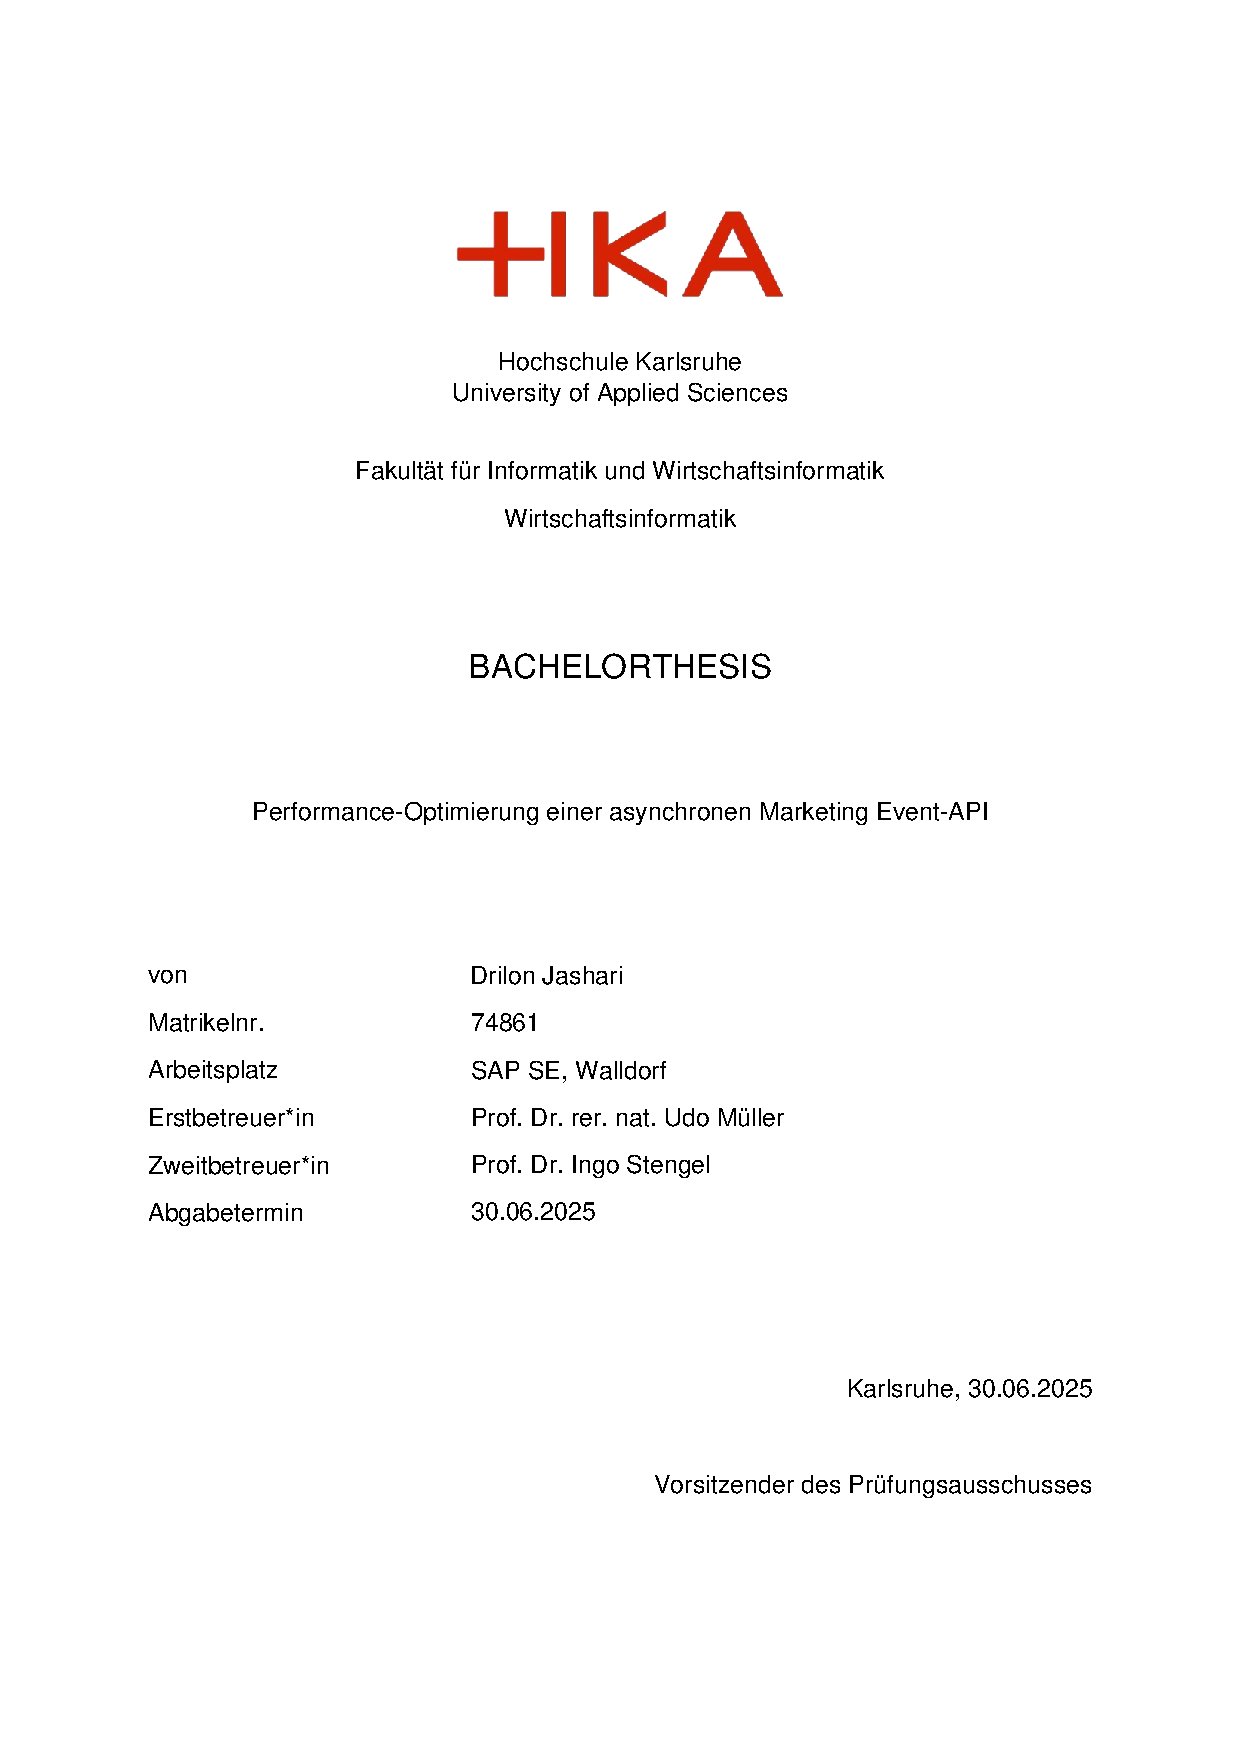
\includepdf[pages=1]{Deckblatt.pdf}

% Inhaltsverzeichnis
\tableofcontents
\clearpage

% Hauptkapitel
\chapter{Einleitung}
\section{Problemstellung und Motivation}
\section{Forschungsfrage und Hypothesen}
\section{Zielsetzung und Abgrenzung}
\section{Aufbau der Arbeit}

\chapter{Theoretische Grundlagen}
\section{Marketing-Automatisierung und Event-APIs}
\section{Java: Architektur, Speicherverwaltung und Threading-Modell}
\section{Node.js: Event-Loop, asynchrone Programmierung}
\section{Leistungsmessung von Webdiensten: Methoden und Metriken}

\chapter{Stand der Forschung}
\section{Bestehende Vergleiche zwischen Java und Node.js}
\section{Performance-Optimierung von Web-APIs}
\section{Spezifische Herausforderungen bei Marketing-Event-APIs}

\chapter{Methodik}
\section{Beschreibung der untersuchten Systeme}
\section{Entwicklungs- und Testumgebung}
\section{Erhebungsmethoden und Metriken}
\section{Teststrategie und Lastprofile}

\chapter{Implementierung}
\section{Java-Implementierung: Architektur und Besonderheiten}
\section{Node.js-Migration: Anpassungen und Herausforderungen}
\section{Optimierungsstrategien}

\chapter{Ergebnisse}
\section{Darstellung der Messergebnisse}
\section{Vergleich beider Implementierungen}
\section{Analyse der Leistungsunterschiede}

\chapter{Diskussion}
\section{Interpretation der Ergebnisse}
\section{Beantwortung der Forschungsfrage}
\section{Kritische Würdigung der Methodik}
\section{Praktische Implikationen für SAP Emarsys}

\chapter{Fazit und Ausblick}
\section{Zusammenfassung der Ergebnisse}
\section{Praktische Empfehlungen}
\section{Weiterführende Forschungsfragen}

% Literaturverzeichnis
\bibliographystyle{plain}
\bibliography{literatur}

% Anhang
\appendix
\chapter{Anhang}
\section{Quellcode-Auszüge}
\section{Detaillierte Messergebnisse}
\section{Sonstige relevante Materialien}

\end{document}